\documentclass[sigconf]{acmart}

\settopmatter{printacmref=false}
\renewcommand\footnotetextcopyrightpermission[1]{}
\pagestyle{plain}

\usepackage{amsmath}
\usepackage{bm}
\usepackage{nicefrac}
\usepackage{booktabs}
\usepackage{array}
\usepackage{multirow}
\usepackage{threeparttable}
\usepackage{makecell}
\usepackage[procnumbered,ruled,vlined,linesnumbered]{algorithm2e}
\usepackage{siunitx}
\usepackage{stfloats}
\usepackage{graphicx}
\usepackage{subfigure}
\usepackage{hyperref}
\usepackage{array}
\usepackage{epstopdf}
\usepackage{balance}
\usepackage{tabularx}
\usepackage{stfloats}
\usepackage{lipsum}

\newtheorem{problem}{Problem}
\newtheorem{theorem}{Theorem}[section]
\newtheorem{corollary}[theorem]{Corollary}
\newtheorem{lemma}[theorem]{Lemma}
\newtheorem{definition}[theorem]{Definition}
\newtheorem{fact}[theorem]{Fact}

% \newcommand{\proof}{{\bf Proof.}\hskip 0.3truecm}
% \newcommand{\endproof}{\quad \(\Box\)}

\newcommand{\defeq}{\stackrel{\mathrm{def}}{=}}
\newcommand{\setof}[1]{\left\{#1 \right\}}
% \newcommand{\sizeof}[1]{\left|#1 \right|}
\newcommand{\abs}[1]{\left|#1 \right|}
\newcommand{\mean}[1]{\mathbb{E}[#1]}
\newcommand{\ceil}[1]{\left\lceil#1\right\rceil}
\newcommand{\Abs}[1]{\left\Vert#1\right\Vert}
\newcommand{\trace}[1]{\mathrm{Tr}\left(#1\right)}

\newcommand{\bsym}[1]{\boldsymbol{#1}}
\newcommand{\myord}[1]{{#1}^{\rm{th}}}
\newcommand{\rea}{\mathbb{R}}
\newcommand{\gr}{\mathcal{G}}
\newcommand{\vecd}{\bsym{d}}
\newcommand{\veca}{\bsym{a}}
\newcommand{\vecb}{\bsym{b}}
\newcommand{\vece}{\bsym{e}}
\newcommand{\allone}{\bsym{1}}
\newcommand{\vecl}{\bsym{l}}
\newcommand{\vecv}{\bsym{v}}
\newcommand{\vecpi}{\bsym{\pi}}
\newcommand{\vecx}{\bsym{x}}

\newcommand{\pscr}{\mathscr{P}}

\newcommand{\lap}{\bsym{L}}
\newcommand{\matd}{\bsym{D}}
\newcommand{\mata}{\bsym{A}}
\newcommand{\matb}{\bsym{B}}
\newcommand{\matw}{\bsym{W}}
\newcommand{\matp}{\bsym{P}}
\newcommand{\matpcal}{\bsym{\mathcal{P}}}
\newcommand{\matf}{\bsym{F}}
\newcommand{\matfstar}{\bsym{F}^*}
\newcommand{\mati}{\bsym{I}}
\newcommand{\matq}{\bsym{Q}}
\newcommand{\matr}{\bsym{R}}
\newcommand{\mats}{\bsym{S}}
\newcommand{\matx}{\bsym{X}}
\newcommand{\maty}{\bsym{Y}}
\newcommand{\matz}{\bsym{Z}}
\newcommand{\matpi}{\bsym{\Pi}}

\newcommand{\lemref}[1]{Lemma~\ref{#1}}
\newcommand{\thmref}[1]{Theorem~\ref{#1}}
\newcommand{\probref}[1]{Problem~\ref{#1}}
\newcommand{\algoref}[1]{Algorithm~\ref{#1}}
\newcommand{\defref}[1]{Definition~\ref{#1}}
\newcommand{\secref}[1]{Section~\ref{#1}}
\newcommand{\tabref}[1]{Table~\ref{#1}}
\newcommand{\figref}[1]{Figure~\ref{#1}}

\newcommand{\edge}[2]{\langle #1, #2 \rangle}


\DeclareMathOperator*{\argmin}{arg\,min}
\DeclareMathOperator*{\argmax}{arg\,max}

\DontPrintSemicolon
\SetKw{KwAnd}{and}
\SetFuncSty{textsc}
\SetKwInOut{Input}{Input\ \ \ \ }

\SetKwInOut{Output}{Output}

\begin{document}
\sloppy
\fancyhead{}
\title{MANC: A Node Group Centrality Based on Absorbing Random Walk}
\author{Haisong Xia and Zhongzhi Zhang \footnotemark}
\affiliation{
    \institution{Shanghai Key Laboratory of Intelligent Information Processing, Fudan University, Shanghai 200433, China\\
        School of Computer Science, Fudan University, Shanghai 200433, China}
    \city{}\country{}
}
\email{{hsxia18,zhangzz}@fudan.edu.cn}
\begin{abstract}
    In the field of complex networks, the problem of important node discovery is increasingly becoming one of the important topics of academic research.
    % Although a large number of node centrality-related studies have been conducted previously, most of the existing studies focus only on the centrality of single node in the network, which are inadequate when applied to multiple important node discovery problems. 
    In this paper, we extend the hitting time of a single node to the case of multiple nodes based on absorbing random walk.
    Specifically, we define a new metric related to the set of absorbing nodes: Multiple Absorbing Node Centrality(MANC).
    For undirected graphs, MANC for a node set \(S\) is defined as the weighted average of the hitting times of absorbing random walks from all nodes in the graph to \(S\).
    Based on the new metric, we construct MANC minimization problem: return the optimal set \(S^*\) of absorbing nodes with capacity \(k\), which minimize its MANC \(M(S^*)\).
    In this paper, we prove that this problem is NP-hard. However, thanks to the monotonicity and supermodularity of MANC, we give greedy algorithms with a \(1-\frac{1}{e}\) approximate factor and cubic running time.
    To accelerate the computation of MANC by avoiding the time-consuming matrix inversion, we give a faster algorithm with a \(1-\frac{1}{e}-\epsilon\) approximate factor and nearly linear running time for any \(\epsilon>0\). Numerical experiments on large-scale real networks demonstrate that our second algorithm is still well scalable while maintaining the approximation error.
\end{abstract}
\keywords{social network, random walk, graph algorithm, Laplacian solver}
\maketitle
\renewcommand{\thefootnote}{*}
\footnotetext[1]{Corresponding author. Zhongzhi Zhang is also with Shanghai Blockchain Engineering Research Center, as well as Research Institute of Intelligent Complex Systems, Fudan University, Shanghai 200433.}

\section{Introduction}

Among all the topics in the field of network science and graph mining, the problem of identifying important nodes has been heavily studied.
Due to the small-world and scale-free properties of complex networks, changes in a very few nodes may have a tremendous impact on the entire network.
This feature can also be verified in real-life situations such as the spread of virus, community opinion impact, and power grid collapse.
If we are able to identify the most critical or vulnerable nodes in a network, then we can take effective preventive measures in advance to avoid unnecessary huge cost.
Therefore, the problem of identifying important nodes also has high research value.

While a large number of node centrality-related studies have been conducted previously, most of the existing studies focus only on the centrality of single node in the network, which are inadequate when applied to multiple important node discovery problems.
For example, removing an important node in a network may result in significant changes in the importance of the remaining nodes.
Therefore, the traditional important node ranking algorithm has good recognition accuracy only for nodes with the highest centrality, and has limitations in solving the problem of identifying important nodes in practice.
The centrality defined for node groups, on the other hand, considers the impact on the network after removing multiple nodes at the same time.
It can better adapt to different scenarios in practical applications while improving the accuracy of identification.

Meanwhile, random walk on graphs is widely applicated in many fields due to its recursiveness and robustness: from link prediction~\cite{YiGuWeTiHa10} and improving search results~\cite{LiPeMaQiWeQi10}, which are closely related to complex networks, to object detection~\cite{GoViHuRa10}, image background extraction~\cite{HuWaYeChLa16} and image annotation refinement~\cite{WaJiZhZh10} in image processing, to DDoS attack detection~\cite{XuZhXiYu14} and clone attack detection~\cite{ZeCaZhGuXi10} in the field of information security.
In this paper, we establish a metric relevant to node group centrality: Multiple Absorbing Node Centrality (MANC) through an absorbing random walk model on graphs.
For a connected undirected graph, the MANC \(M(S)\) of a node set \(S\) is defined as the weighted average of the hitting times of absorbing random walks from all nodes in the graph to \(S\).

Due to the definition of MANC, this metric can be directly applied to the search engine ranking systems.
If we denote web page that satisfy the search keywords as nodes, and denote hyperlinks between web pages as edges, the selected set of web pages should be close enough to all candidate pages, i.e. cover all candidate pages as much as possible.
The traditional method of ranking important nodes cannot meet the above requirements, while MANC can theoretically achieve better application results because it is defined directly according to the hitting time of node group.
Consequently, we further construct the MANC minimization problem: finding the node set \(S^*\) with capacity \(k\) that minimizes MANC \(M(S^*)\).

In this paper, we prove that the MANC minimization problem is NP-hard.
Subsequently, we use the monotonicity and supermodularity of MANC to design greedy algorithms with approximation guarantees to solve this problem.
However, the inevitable matrix inversion in the greedy algorithm leads to a complexity of \(O(kn^3)\) for networks containing \(n\) nodes, which cannot be employed in large networks.
Then, we attempt to reformulate MANC as the quadratic form of the inverse of a SDDM matrix so that we can approximate it by using SDD solver~\cite{CoKyMiPaJaPeRaXu14,SpTe14} and Johnson-Lindenstrauss Lemma~\cite{JoLi84}.
For network with \(n\) nodes and \(m\) edges, our proposed fast greedy algorithm \textsc{Approx} has a \(\tilde{O}(km)\) time complexity.
In order to verify the accuracy and efficiency of \textsc{Approx}, we perform extensive numerical experiments on networks of different sizes, the result demonstrates that \textsc{Approx} is still well scalable while maintaining the approximation error and can be applicated in large networks with millions of nodes.
% \subsection{Related Works}

\section{Preliminary}

In this section, we briefly indroduce some notations as well as some basic concepts on graphs, random walk and special functions.

\subsection{Notations}

In the rest of the paper, we distinguish scalars, vectors and matrices by using regular lowercase letters \(a,b,c\), bold lowercase letters \(\veca,\bsym{b},\bsym{c}\) and bold uppercase letters \(\mata,\bsym{B},\bsym{C}\) respectively.
For the convenience of representing some specific elements in vectors and matrices, we use \(\veca_{i}\) to denote the \(\myord{i}\) entry of vector \(\bsym a\) and \(\bsym A_{[i,j]}\) to denote entry \((i,j)\) of matrix \(\bsym A\).
We also use \(\mata_{[i,:]}\) and \(\mata_{[:,j]}\) to respectively denote the \(\myord{i}\) row and the \(\myord{j}\) column of matrix \(\mata\).

Moreover, to facilitate the representation of subvectors and submatrices, we introduce sets in the subscripts of vectors and matrices.
For example, let \(S=\setof{S_1,S_2,\dots,S_t}\), we use \(\veca_{-S}\) to denote the subvector of \(\veca\) obtained by removing the \(\myord{S_1},\myord{S_2},\dots,\myord{S_t}\) component.
We also use \(\mata_{-S}\) to denote the submatrix of \(\mata\) obtained by removing elements that either in the \(\myord{S_1},\myord{S_2},\dots,\myord{S_t}\) row or in the \(\myord{S_1},\myord{S_2},\dots,\myord{S_t}\) column.

Note that when a vector or matrix has both superscripts and subscripts, the subscript takes precedence over the superscript.
Therefore, \(\mata_{-S}^{-1}\) denotes the inverse of \(\mata_{-S}\) rather than the submatrix of \(\mata^{-1}\). Finally, we use \(\bsym{e}_i\) to denote the \(\myord{i}\) standard basis vector of particular dimensions, and \(\allone_n\in \rea^n\) to denote a vector of \(n\) dimensions with all elements of \(1\). Sometimes, we omit subscripts where there is no ambiguity.

\subsection{Graphs and Laplacian Matrices}\label{sub:lap}

In the rest of the paper, we use \(\gr=(V,E,w)\) to denote connected weighted undirected graph with \(n=\abs{V}\) nodes and \(m=\abs{E}\) edges, where \(V,E\) denote the node set and edge set of \(\gr\) respectively, and \(w:E\to\rea^+\) denote the edge weight function.
We use \(e=\edge{u}{v}\) to represent an edge \(e\) connecting node \(u\) and node \(v\), and also use \(w_{\min}\) and \(w_{\max}\) to represent the minimum and maximum edge weight of \(\gr\) respectively, thus, \(w_{\min}=\min_{e\in E}w_e\),\(w_{\max}=\max_{e\in E}w_e\).

After giving the denotation of \(\gr\), then the adjacency matrix of \(\gr\) can be denoted as \(\mata\in \rea^{n\times n}\): for node \(i,j\in V\), \(\mata_{[i,j]}=\mata_{[j,i]}=w_{i,j}\) if \(i\) and \(j\) are adjacent, and \(\mata_{[i,j]}=\mata_{[j,i]}=0\) otherwise.
Moreover, degree \(\vecd_i\) of node \(i\) can be defined as \(\vecd_i=\sum_{j=1}^n\mata_{[i,j]}\).
If we denote the relevant degree diagnoal matrix as \(\matd={\rm{diag}}(\vecd)\), then the Laplacian matrix \(\lap\) of \(\gr\) is \(\lap=\matd-\mata\).

The Laplacian matrix of a graph has other definitions.
For an undirected graph \(\gr\), we first assign an arbitary direction to each edge in \(\gr\), then for edge \(e=\edge{i}{j}\in E\), the row corresponding to edge \(e\) in the incidence matrix \(\matb\in\rea^{m\times n}\) of \(\gr\) can be denoted as \(\matb_{[e,:]}=e_i-e_j\).
Furthermore, let \(\matw\in\rea^{m\times m}\) be a diagnoal matrix whose diagnoal entry \((e,e)\) is denoted as \(w_e\), then the Laplacian matrix \(\lap\) of \(\gr\) can be defined as \(\lap=\matb^\top\matw\matb=\sum_{e\in E}w_e\bsym{b}_e\bsym{b}_e^\top\).
From the definition above, it is easy to prove that \(\lap\) is positive semi-definite.

\subsection{Random Walk on Graphs}

For a connected weighted graph \(\gr\), the classical random walk model of \(\gr\) can be described by the transition matrix \(\matp\): at any time step, the walker located at node \(i\) moves to node \(j\) with probability \({\matp_{[i,j]}=\mata_{[i,j]}}/{\vecd}_i\).
It is easy to verify that

\begin{equation}\label{eq:trs}
    \matp=\matd^{-1}\mata
\end{equation}

If \(\gr\) is non-bipartite and finite, there exists a unique stationary distribution of the random walk
\[
    \vecpi=\begin{pmatrix}
        \pi_1 & \pi_2 & \dots & \pi_n
    \end{pmatrix}^\top=\begin{pmatrix}
        \frac{\vecd_1}{d} & \frac{\vecd_2}{d} & \dots & \frac{\vecd_n}{d}
    \end{pmatrix}^\top
\]
where \(d=\sum_{i=1}^n\vecd_i\).

Let \(X_{u,t}^r\) denote the location of random walker \(r\) starting from node \(u\) at time step \(t\), then we can give the definition of hitting time, also known as absorb length, which is a fundamental quantity in random walks.

\begin{definition}[Hitting Time]
    The hitting time \(T_{u,S}\) from node \(u\) to node set \(S\) is the expected number of time steps for a walker starting from \(u\) to visit an arbitary node of \(S\) for the first time. Therefore, \(T_{u,S}\) can be written as
    \[T_{u,S}^r=\min\{t:X_{u,t}\in S,t\ge0 \}\]
    \[T_{u,S}=\mean{T_{u,S}^r}\]
\end{definition}

\subsection{Supermodular Functions}

Subsequently, we give the definitions of monotone and supermodular set functions. For simplicity, we denote \(S\cup\{u\}\) as \(S+u\).

\begin{definition}[Monotonicity]
    The set function \(f:2^{V}\to\rea^+\) is monotone if and only if \(\forall X\subseteq Y\subseteq V\) satisfies \(f(X)\ge f(Y)\).
\end{definition}

\begin{definition}[Supermodularity]
    The set function \(f:2^{V}\to\rea^+\) is supermodular if and only if \(\forall X\subseteq Y\subseteq V, u\in V\setminus Y\) satisfies \(f(X)-f(X+u)\ge f(Y)-f(Y+u)\).
\end{definition}

\section{Problem Formulation}

\subsection{Definition of MANC and Its Minimization Problem}

In this paper, we define Multiple Absorbing Node Centrality (MANC) \(M(S)\) as the weighted average of the hitting times of absorbing random walks from all nodes in the graph to \(S\).

\begin{definition}[MANC]\label{def:manc}
    \[M(S)=\sum_{u\in V}\vecpi_u T_{u,S}=\sum_{u\in V}\vecpi_u \mean{\min\{t:X_{u,t}^r\in S,t\ge0\}}\]
\end{definition}

The definition of MANC naturally raises the problem of minimizing MANC subject to a cardinality constraint.

\begin{problem}[Multiple Absorbing Node Centrality Minimization, MANCM]
Given a connected undirected graph \(\gr=(V,E,w)\) with \(n\) nodes, \(m\) edges and an integer \(k\in[1,n]\), the goal is to find a node set \(S^*\subseteq V\) such that MANC \(M(S^*)\) is minimized:
\[S^*=\argmax_{S\subseteq V,\abs{S}=k}M(S)\]
\end{problem}

According to ~\cite{KeSn76}, we are able to transfrom the definition of MANC into the inverse of SDDM matrix.

\begin{fact}
    Given the absorbing node set \(S\) and transition matrix \(\matp\), then the fundamental matrix \(\matf\) can be denoted as
    \begin{equation}\label{eq:funda}
        \matf=\sum_{l=0}^\infty\matp_{-S}^l=(\mati-\matp_{-S})^{-1}=(\mati-\matp)_{-S}^{-1}
    \end{equation}
\end{fact}

According to ~\eqref{eq:funda}, the entry \((i,j)\) of \(\matf\) can be represented as the expected number of passages through node \(j\) by the random walker starting from node \(i\) before being absorbed.
From the linearity of mean, it follows that the hitting time of a random walker is equivalent to the sum of the expected number of passages through all nodes in the graph, i.e. \(\vecl=\matf\allone\), where \(\vecl_i\) denotes the hitting time of a random walker starting from node \(i\).
In particular, if the random walker starts from absorbing node, the hitting time can be regarded as \(0\). Considering the above case, MANC \(M(S)\) can be written as
\[M(S)=\vecpi_{-S}^\top\vecl=\vecpi_{-S}^\top\matf\allone=\vecpi_{-S}^\top(\mati-\matp)_{-S}^{-1}\allone\]

Furthermore, after simplification using ~\eqref{eq:trs}, we get the formula of \(M(S)\):
\begin{equation}\label{eq:MANC}
    \begin{split}
        M(S) & =\vecpi_{-S}^\top\left(\mati-\matp\right)_{-S}^{-1}\allone                                    \\
        & =\vecpi_{-S}^\top\left(\mati-\matd^{-1}\mata\right)_{-S}^{-1}\allone                          \\
        & =\vecpi_{-S}^\top\left(\mati-\matd^{-1}\mata\right)_{-S}^{-1}\matd_{-S}^{-1}\matd_{-S}\allone \\
        & =\vecpi_{-S}^\top\left(\matd-\mata\right)_{-S}^{-1}\vecd_{-S}                                \\
        & =\vecpi_{-S}^\top\lap_{-S}^{-1}\vecd_{-S}
    \end{split}
\end{equation}

\subsection{Physic Explanations of MANC}

After detailing MANC and MANCM, we try to establish a connection between MANC \(M(S)\) and extra detour time \(\Delta D_{i,j}(S)\), which enables us to understand the importance of node set \(S\) from a different perspective. The similar idea of extra detour time has been proposed in~\cite{RaGyZh13}, where the authors prove a equation related to topological centrality and extra detour time of a single node. In this paper, we try to explore the detour time of a node set instead of a single node, giving a physical explanation of MANC.

Random detour time \(D_{i,j}(S)\) is a natural extension of hitting time when considering random walk on a graph, which is defined as the expected time of a walker who starts from node \(i\), must visit an arbitary node in set \(S\), then first reaches node \(j\). Consequently, extra detour time \(\Delta D_{i,j}(S)\) is defined as the difference between random detour time and hitting time, i.e. \(\Delta D_{i,j}(S)=D_{i,j}(S)-T_{i,j}\). It is intuitive that the larger \(\Delta D_{i,j}(S)\) is ,the harder it is for a walker to reach nodes in \(S\), and less important \(S\) is in the whole network. Actually, we can prove the following theorem, which confirms the connection between MANC \(M(S)\) and extra detour time \(\Delta D_{i,j}(S)\).

\begin{theorem}\label{thm:extra_detour}
    \begin{equation}\label{eq:extra-detour}
        M(S)=\sum_{i=1}^n\sum_{j=1}^n\vecpi_i\vecpi_j\Delta D_{i,j}(S)
    \end{equation}
\end{theorem}
\begin{proof}
    % \(\matfstar={(\mati-\matp+\allone\vecpi^\top)}^{-1}\matpi^{-1}\)
    To prove equation~\eqref{eq:extra-detour}, we utilize the fundamental matrix \(\matfstar\) in the non-absorbing random walk.
    According to~\cite{BoRaZh11}, \(\matfstar\) can be represented as \(\matfstar=(\mati-\matp+\allone\vecpi^\top)^{-1}\matpi^{-1}\).
    Subsequently, the hitting time \(H_{i,j}\) can be represented by \(\matfstar\) as \(H_{i,j}=\matfstar_{[j,j]}-\matfstar_{[i,j]}\).
    If we denote the probability that a walker starting from node \(i\) first reaches node \(u\) in absorbing set \(S\) as the \(\myord{(i,u)}\) entry of matrix \(\matpcal\in\rea^{n\times\abs{S}}\), then we can use \(\matfstar\) to represent the weighted average of random detour time as
    \begin{align*}
        \sum_{i=1}^n\sum_{j=1}^n\vecpi_i\vecpi_jD_{i,j}(S)
         & =\sum_{i=1}\vecpi_i T_{i,S}+\sum_{i=1}^n\sum_{j=1}^n\sum_{k=1}^{\abs{S}}\vecpi_i\vecpi_j\matpcal_{[i,k]}T_{k,j}  \\
         & =M(S)+\sum_{j=1}^n\vecpi_j\vecpi^\top\matpcal(\matfstar_{[j,j]\allone-\matfstar_{[S,j]}})                        \\
         & =M(S)+\sum_{j=1}^n\vecpi_j\matfstar_{[j,j]}\vecpi^\top\matpcal\allone-\vecpi^\top\matpcal\matfstar_{[S,:]}\vecpi \\
         & =M(S)+\sum_{j=1}^n\vecpi_j\matfstar_{[j,j]}-1
    \end{align*}
    where the last equality is due to the fact that \(\matpcal\allone=\allone\) and \(\matfstar\vecpi=\allone\).
    Afterwards, we are able to rewrite the right hand side of equation~\eqref{eq:extra-detour} as
    \begin{align*}
        \sum_{i=1}^n\sum_{j=1}^n\vecpi_i\vecpi_j\Delta D_{i,j}(S)
         & =\sum_{i=1}^n\sum_{j=1}^n\vecpi_i\vecpi_jD_{i,j}(S)-\sum_{i=1}^n\sum_{j=1}^n\vecpi_i\vecpi_jT_{i,j}         \\
         & =M(S)+\sum_{j=1}^n\vecpi_j\matfstar_{[j,j]}-1-\sum_{i=1}^n\sum_{j=1}^n(\matfstar_{[j,j]}-\matfstar_{[i,j]}) \\
         & =M(S)+\sum_{j=1}^n\vecpi_j\matfstar_{[j,j]}-1-(\sum_{j=1}^n\vecpi_j\matfstar_{[j,j]}-1)                     \\
         & =M(S)
    \end{align*}
    which completes our proof.
\end{proof}

\subsection{Properties of MANC}

After proposing physic explanations of MANC, we attempt to study the properties of them. First, we prove that MANCM is NP-hard.
Subsequently, we prove that the set function \(M(\cdot)\) is monotone and supermodular, which provides us with a theorecical basis for designing greedy algorithms with approximation guarantees.

\subsubsection{NP-hard}

\

To prove the NP-hardness of MANCM, we first give the detailed definition of vertex cover and a decision version of MANCM, trying to construct a reduction from the former to the latter on \(c\)-regular graphs.

\begin{problem}[Vertex Cover on \(c\)-regular graphs]
Given a connected \(c\)-regular graph \(G=(V,E)\) and an integer \(k\), the goal is to find out whether there exists a node set \(S\subseteq V\) such that \(\abs{S}\le k\) and every edge in \(E\) is incident with at least one node in \(S\).
\end{problem}

\begin{problem}[Multiple Absorbing Node Centrality Minimization, Decision Version, MANCMD]
Given a connected weighted graph \(\gr=(V,E,w)\), a real number \(b\) and an interger \(k\).
The goal is to find out whether there exists a node set \(S\subseteq V\) such that \(\abs{S}\le k\) and \(M(S)\le b\).
\end{problem}

\begin{lemma}\label{lem:reduct}
    Let \(\gr=(V,E,w)\) be a connected \(c\)-regular graph graph with all edge weights being \(1\).
    Let \(S\subseteq V\) be a nonempty node set with capacity \(k\), then \(M(S)\ge (n-k)/n\) and the equality holds if and only if \(S\) is a vertex cover of \(\gr\).
\end{lemma}
\begin{proof}
    We first prove that if \(S\) is a vertex cover of \(\gr\), then \(M(S)=(n-k)/n\).
    When \(S\) is a vertex cover of \(\gr\), because there are no edges between nodes in \(V\setminus S\), we can simplify~\eqref{eq:MANC} as
    \[M(S)=\vecpi_{-S}^\top\lap_{-S}^{-1}\vecd_{-S}=\vecpi_{-S}^\top\matd_{-S}^{-1}\vecd_{-S}=\vecpi_{-S}^\top\allone\]
    Since \(\gr\) is a \(c\)-regular graph, \(\vecpi=\begin{pmatrix}1/n&\cdots&1/n\end{pmatrix}^\top\).
    Thus, \(M(S)=\vecpi_{-S}^\top\allone=(n-k)/n\).

    We then prove that if \(S\) is not a vertex cover of \(\gr\), then \(M(S)>(n-k)/n\).
    For node \(u\in S\) and node \(v\in V\setminus S\), it is obvious that \(\Pr(T_{u,S}^r=0)=\Pr(T_{v,S}^r\neq0)=1\).
    Meanwhile, because \(S\) is not a vertex cover of \(\gr\), edge set \(E\) has at least one edge \((u',v')\) that is not covered by \(S\).
    Let \(d_{\max}=\max\{d_u|u\in V\}\),\(v\in V\setminus(S+u'+v')\), then we get
    \[\Pr(T_{v,S}^r=1)-\Pr(T_{u',S}^r=1)>\frac{1}{d_{\max}}>\frac{1}{n}\]
    \[\Pr(T_{v,S}^r=1)-\Pr(T_{v',S}^r=1)>\frac{1}{d_{\max}}>\frac{1}{n}\]

    Therefore, we are able to give a lower bound of hitting time for nodes \(u'\),\(v'\) and node \(v\in V\setminus(S+u'+v')\).
    \[\mean{T_{u,S}^r}\ge1\]
    \[\mean{T_{u',S}^r}=\mean{T_{v',S}^r}\ge(1-\frac1n)+2\times\frac1n=1+\frac1n\]

    Therefore, we finally get the lower bound of MANC:
    \begin{align*}
        M(S) & =\sum_{v\in V}\vecpi_v\mean{T_{v,S}^r}                                                                             \\
             & =\sum_{v\in V\setminus(S+u'+v')}\vecpi_v\mean{T_{v,S}^r}+\vecpi_{u'}\mean{T_{u',S}^r}+\vecpi_{v'}\mean{T_{v',S}^r} \\
             & \ge\vecpi_{-(S+u'+v')}\allone+\vecpi_{u'}(1+\frac1n)+\vecpi_{v'}(1+\frac1n)                                        \\
             & =\vecpi_{-S}^\top\allone+\frac{\vecpi_{u'}+\vecpi_{v'}}n
        >\vecpi_{-S}^\top\allone=(n-k)/n
    \end{align*}
\end{proof}

After accomplishing the proof of \lemref{lem:reduct}, we prove that MANCM is NP-hard based on it.
\begin{theorem}\label{thm:np-hard}
    MANCM is NP-hard.
\end{theorem}
\begin{proof}
    we prove the NP-hardness of MANCM by constructing a polynomial reduction from Vertex Cover to MANCMD.
    \[p:\{(G=(V,E),k)\}\to\{(\gr=(V,E,w),k,b)\}\]
    For connected graph \(G=(V,E)\) with \(n\) nodes, we construct a new graph \(G'=(V,E,w')\), where the node set and edge set are identical to those in \(G\), and the weight function on the edge set is defined as \(w':E\to\{1\}\), i.e. the weights of all edges are equal to \(1\). Then we can construct a reduction as
    \[p((G=(V,E),k))=(G'=(V,E,w'),k,\vecpi_{-S})\]
    According to~\lemref{lem:reduct}, \(p\) is a polynomial reduction from Vertex Cover to MANCMD, which completes our proof.
\end{proof}

\subsubsection{Monotonicity and Supermodularity}

\

In this part, we prove that the objective function \(M(\cdot)\) is monotone and supermodular.
\begin{theorem}[Monotonicity]\label{thm:mono}
    Let \(S\) be an arbitary nonempty node set of connected weighted graph \(\gr=(V,E,w)\), then for node \(u\in V\setminus S\),
    \[M(S)\ge M(S+u)\]
\end{theorem}

\begin{proof}
    According to \defref{def:manc}, \(M(S)=\sum_{v\in V}\vecpi_v\mean{T_{v,S}^r}\). Since \(S\) is a subset of \(S+u\), when a random walker reaches nodes in \(S\), it must have reached nodes in \(S+u\), i.e. \(T_{v,S}^r\ge T_{v,S+u}^r\). Therefore \(\mean{T_{v,S}^r}\ge\mean{T_{v,S+u}^r}\) holds for any node \(v\in V\), which completes our proof.
\end{proof}

\begin{theorem}[Supermodularity]\label{thm:supermod}
    Let \(S,T\) be arbitary nonempty node sets of connected weighted graph \(\gr=(V,E,w)\) such that \(S\subseteq T\subsetneq V\), then for node \(u\in V\setminus T\),
    \[M(S)-M(S+u)\ge M(T)-M(T+u)\]
\end{theorem}

\begin{proof}
    For a subset \(A\) of the probability space, we denote \(\allone_A\) as the indicator function of the event \(A\). Then we rewrite \(M(S)-M(S+u)\) by discussing the hitting node of random walker.
    \begin{align*}
        M(S)-M(S+u)
        = & \sum_{v\in V}\vecpi_v\left(\mean{T_{v,S}^r}-\mean{\min\{T_{v,S}^r,T_{v,u}^r \}}\right)      \\
        = & \sum_{v\in V}\vecpi_v(\mean{T_{v,S}^r}-\mean{T_{v,S}^r\allone_{\{T_{v,S}^r\le T_{v,u}^r\}}} \\
          & -\mean{T_{v,S}^r\allone_{\{T_{v,u}^r<T_{v,S}^r\}}})                                         \\
        = & \sum_{v\in V}\vecpi_v\mean{(T_{v,S}^r-T_{v,u}^r)\allone_{\{T_{v,u}^r<T_{v,S}^r\}}}
    \end{align*}
    Similarly, we also have
    \[M(T)-M(T+u)=\sum_{v\in V}\vecpi_v\mean{(T_{v,T}^r-T_{v,u}^r)\allone_{\{T_{v,u}^r<T_{v,T}^r\}}}\]
    As is mentioned in proof of \thmref{thm:mono}, \(T_{v,S}^r\ge T_{v,T}^r\forall v\in V\).
    It is also obvious that \(\allone_{\{T_{v,u}-T_{v,S}\}}\ge\allone_{\{T_{v,u}-T_{v,T}\}}\).
    Combining the above two inequalities, we can prove that
    \[(T_{v,S}^r-T_{v,u}^r)\allone_{\{T_{v,u}^r<T_{v,S}^r\}}\ge(T_{v,T}^r-T_{v,u}^r)\allone_{\{T_{v,u}^r<T_{v,T}^r\}}\]
    holds for any node \(v\in V\), which completes our proof.
\end{proof}

\section{Simple Greedy Algorithm}

Due to the monotonicity and supermodularity of the set function \(M(\cdot)\), there exists a simple greedy algorithm with a \(1-\frac1e\) approximate factor to MANCM~\cite{NeWoFi78}:
At each iteration, a new absorbing node \(u^*\) is selected from the set of non-absorbing nodes \(V\setminus S\), satisfying
\[margin(u,S)=M(S)-M(S+u)\]
\[u^*=\argmax_{u\in V\setminus S}(margin(u,S))\]

It is easy to find that the simple algorithm above needs to compute \(margin(u,S)\) for each node \(u\) in the graph at each iteration, leading to \(O(n)\) matrix inverse operations.
When using the naive matrix inverse algorithm with complexity \(O(n^3)\), the overall complexity of the simple greedy algorithm is \(O(kn^4)\).
By simplifying \(margin(u,S)\), we attempt to reduce the time complexity of greedy algorithm.

For node \(u\in V\setminus S\), after adjusting the order of submatrix \(\lap_{-S}\), we rewrite \(\lap_{-S}\) as
\[\lap_{-S}=\begin{pmatrix}l_u & -\veca^\top \\-\vecb&\mata\end{pmatrix}\]
where \(\mata\) denotes \(\lap_{-(S+u)}\).
According to the properties of block matrices, we can get
\[\lap_{-S}^{-1}=\begin{pmatrix}
        t & t\veca^\top\mata^{-1} \\t\mata^{-1}\vecb&\mata^{-1}+t\mata^{-1}\vecb\veca^\top\mata^{-1}
    \end{pmatrix}\]
where \(t=(l_u-\veca^\top\mata^{-1}\veca)^{-1}\).
Therefore, when \(S\neq\varnothing\), \(margin(u,S)\) can be rewritten as

\begin{equation}\label{eq:margin-deriv}
    \begin{split}
        &M(S)-M(S+u)\\
        =&\vecpi_{-S}^\top\lap_{-S}^{-1}\vecd_{-S}-\vecpi_{-(S+u)}^\top\lap_{-(S+u)}^{-1}\vecd_{-(S+u)}\\
        =&\begin{pmatrix}\vecpi_u&\vecpi_{-(S+u)}^\top\end{pmatrix}\begin{pmatrix}t & t\veca^\top\mata^{-1} \\t\mata^{-1}\vecb&\mata^{-1}+t\mata^{-1}\vecb\veca^\top\mata^{-1}\end{pmatrix}\begin{pmatrix}d_u\\\vecd_{-(S+u)}\end{pmatrix}\\
        &-\vecpi_{-(S+u)}^\top\lap_{-(S+u)}^{-1}\vecd_{-(S+u)}\\
        =&t\vecpi_u\vecd_u+t\vecd_u\vecpi_{-(S+u)}^\top\mata^{-1}\vecb+t\vecpi_u\veca^\top\mata^{-1}\vecd_{-(S+u)}\\
        &+t\vecpi_{-(S+u)}^\top\mata^{-1}\vecb\veca^\top\mata^{-1}\vecd_{-(S+u)}\\
        =&\frac1t(t\vecpi_u+t\vecpi_{-(S+u)}^\top\mata^{-1}\vecb)(td_u+t\veca^\top\mata^{-1}\vecd_{-(S+u)})\\
        =&\frac{(\vecpi_{-S}^\top\lap_{-S}^{-1}\vece_u)(\vece_u^\top\lap_{-S}^{-1}\vecd_{-S})}{\vece_u^\top\lap_{-S}^{-1}\vece_u}=\frac{(\vece_u^\top\lap_{-S}^{-1}\vecd_{-S})^2}{d(\vece_u^\top\lap_{-S}^{-1}\vece_u)}
    \end{split}
\end{equation}

However, when \(S=\varnothing\), equation~\eqref{eq:margin-deriv} is illegal due to the singularity of \(\lap\). Given that \(M(\varnothing)=\infty\), we can define \(margin(u,\varnothing)\) as \(-M(S+u)=-M(\{u\})\), which is the negative of absorbing random-walk centrality for single node \(u\). It is easy to verify that~\cite{ZhXuZh20}

\begin{equation}\label{eq:margin-empty}
    M(\{u\})=d(\vece_u-\vecpi)^\top\lap^\dagger(\vece_u-\vecpi)
\end{equation}

Equation~\eqref{eq:margin-deriv} and equation~\eqref{eq:margin-empty} illustrate that computing \(margin(u,S)\forall u\in V\setminus S\) only requires the inverse of the same matrix \(\lap_{-S}\) or the pseudoinverse of the same matrix \(\lap\) . Consequently, we are able to optimize the simple greedy algorithm as~\algoref{algo:exact}, reducing time complexity from \(O(kn^4)\) to \(O(kn^3)\).

\begin{algorithm}
    \caption{\textsc{Exact}\((\gr,k)\)}
    \label{algo:exact}
    \Input{
        A connected weighted undirected graph \(\gr=(V,E,w)\);
        an integer \(k\in[1,\abs{V}]\)
    }
    \Output{\(S\): A subset of \(V\) with \(\abs{S}=k\)}
    Compute \(\lap\) and \(\vecd\)\;
    \(d\gets\vecd\allone\),\(\vecpi\gets d^{-1}\vecd\)\;
    % \(u^*\gets\argmin_{u\in V}\{d(\vece_u-\vecpi)^\top\lap^\dagger(\vece_u-\vecpi)\}\)\;
    \(S\gets\{\argmin_{u\in V}\{d(\vece_u-\vecpi)^\top\lap^\dagger(\vece_u-\vecpi)\}\}\)\;
    \While{\(\abs{S}<k\)}{
        \ForEach{\(u\in V\setminus S\)}{
            \(margin(u,S)\gets\frac{(\vece_u^\top\lap_{-S}^{-1}\vecd_{-S})^2}{d(\vece_u^\top\lap_{-S}^{-1}\vece_u)}\)\;
        }
        \(u^*\gets\argmax_{u\in V\setminus S}\{margin(u,S)\}\)\;
        \(S\gets S\cup\{u^*\}\)
    }
    \Return{\(S\)}
\end{algorithm}

\section{Faster Greedy Algorithm}

Despite the time complexity optimization made by proposing~\algoref{algo:exact}, this simple greedy algorithm still requires matrix inversion so that it cannot be applicated in large networks. In order to accelerate the computation of~\eqref{eq:margin-deriv} and~\eqref{eq:margin-empty}, we establish efficient approximations of~\eqref{eq:margin-empty}, numerator in~\eqref{eq:margin-deriv} and denominator in~\eqref{eq:margin-deriv} by using~\lemref{lem:JL} and~\lemref{lem:solver}.

\begin{lemma}[Johnson-Lindenstrauss Lemma, JL Lemma~\cite{JoLi84}]\label{lem:JL}
    Given fixed vectors \(\vecv_1,\vecv_2,\dots,\vecv_n\in\rea^d\) and \(\epsilon>0\), let \(\matq\in\rea^{k\times d}\) denote a matrix where \(k\ge\ceil{24\epsilon^{-2}\log n}\), each entry in \(\matq\) is equal to \(1/\sqrt k\) or \(-1/\sqrt k\) with the same probability \(1/2\). Then \(\forall i,j\le n\),
    \begin{equation}\label{eq:JL}
        (1-\epsilon)\Abs{\vecv_i-\vecv_j}^2\le\Abs{\matq\vecv_i-\matq\vecv_j}^2\le(1+\epsilon)\Abs{\vecv_i-\vecv_j}^2
    \end{equation}
\end{lemma}
\lemref{lem:JL} indicates that if we project \(n\) vectors \(\vecv_1,\vecv_2,\dots,\vecv_n\) into a lower dimensional space spanned by \(O(\log n)\) random vectors, the distances between projected vectors will be preserved with high probability.
For the convenience of writing, we will rewrite~\eqref{eq:JL} as\(\Abs{\vecv_i-\vecv_j}^2\approx_\epsilon\Abs{\matq\vecv_i-\matq\vecv_j}^2\) hereinafter.

\begin{lemma}[SDD Solver~\cite{CoKyMiPaJaPeRaXu14,SpTe14}]\label{lem:solver}
    There exists an algorithm \(\vecx=\textsc{Solve}(\mats,\vecb,\delta)\) which takes a SDDM matrix or a Laplacian \(\mats\in\rea^{n\times n}\) with \(\text{nnz}(\mats)=m\), a vector \(\vecb\in\rea^n\), and an error parameter \(\delta>0\) as input, and returns a vector \(\vecx\in\rea^n\) which satisies
    \[\Abs{\vecx-\mats^{-1}\vecb}_{\mats}\le\delta\Abs{\mats^{-1}\vecb}_{\mats}\]
    with high probability.
    Here \(\Abs{\vecx}_{\mats}\) is denoted as \(\sqrt{\vecx^\top\mats\vecx}\), and \(\mats^{-1}\) is denoted as the pseudoinverse of \(\mats\) when \(\mats\) is a Laplacian.
    The expected time complexity of this algorithm is \(\tilde{O}(m)\), where \(\tilde{O}(\cdot)\) omits the poly(\(\log n\)) factors.

\end{lemma}

Based on~\lemref{lem:JL} and~\lemref{lem:solver}, we are able to efficiently approximate the quantities in~\eqref{eq:margin-deriv} and~\eqref{eq:margin-empty} that are related to \(\lap^\dagger\) and \(\lap_{-S}^{-1}\).
Furthermore, we also need the following lemma to provide our approximation.

\begin{lemma}\label{lem:norm-comp}
    Let \(S\subseteq V\) be an arbitary node set of connected weighted graph \(\gr=(V,E,w)\), then for any vector \(\vecv\in\rea^{n-\abs{S}}\),
    \[\vecv_i^2\le n\Abs{\vecv}_{\lap_{-S}}^2\]
\end{lemma}

\subsection{Approximations of~\eqref{eq:margin-empty}}\label{subsec:approx-margin-empty}

Given that~\eqref{eq:margin-empty} can be regarded as the Single Absorbing Node Centrality (SANC), we use an efficient algorithm proposed by~\cite{ZhXuZh20}.
\begin{lemma}\label{lem:approxhk}
    there exists an algorithm with time complexity \(\tilde{O}(m)\), which takes a connected weighted undirected graph \(\gr=(V,E,w)\) and an error parameter \(\epsilon>0\) as input, and returns the approximation \(\tilde{M}(\{u\})\) of SANC \(M(\{u\})\) for any node \(u\) in graph \(\gr\) such that
    \[M(\{u\})\approx_\epsilon\tilde{M}(\{u\})\]
\end{lemma}

\begin{algorithm}
    \caption{\textsc{SANCEst}\((\gr,\epsilon)\)}
    \label{algo:sancest}
    \Input{
        A connected weighted undirected graph \(\gr=(V,E,w)\);
        an error parameter \(\epsilon>0\)
    }
    \Output{The approximation \(\tilde{M}(\{u\})\) of SANC \(M(\{u\})\) for any node \(u\) in graph \(\gr\)}
    Compute \(\lap\) and \(\vecd\)\;
    \(d\gets\vecd\allone\),\(\vecpi\gets d^{-1}\vecd\)\;
    \(k\gets\ceil{24\epsilon^{-2}\log n}\),\(\delta\gets\frac{\epsilon}{6n^2}\sqrt{\frac{(1-\epsilon)w_{\min}}{(1+\epsilon)w_{\max}}}\)\;
    Construct a matrix \(\matq\in\rea^{k\times m}\), each entry of which is \(\pm1/\sqrt k\) with identical probability\;
    Decompose \(\lap\) into \(\matb\in\rea^{m\times n}\) and \(\matw\in\rea^{m\times m}\), where \(\lap=\matb^\top\matw\matb\)\;
    \(\overline{\matx}\gets\matq\matw^{1/2}\matb\)\;
    \For{\(i=1,2,\dots,k\)}{
    \(\matx'_{[i,:]}\gets\textsc{Solve}(\lap,\overline{\matx}_{[i,:]},\delta)\)\;
    }
    \ForEach{\(u\in V\)}{
        \(\tilde{M}(\{u\})\gets d\Abs{\matx'(\vece_u-\vecpi)}^2\)\;
    }
    \Return{\(\{\tilde{M}(\{u\})|u\in V \}\)}

\end{algorithm}

\subsection{Approximations of~\eqref{eq:margin-deriv}}

Before proposing the approximations of~\eqref{eq:margin-deriv}, the proof of the following lemma is necessary.
\begin{lemma}\label{lem:norm-ineq}
    Given a connected weighted undirected graph \(\gr=(V,E,w)\), let \(\lap\) and \(w_{\min}\) denote the Laplacian and the minimal edge weight of the graph respectively.
    Then for an arbitary node set \(S\subseteq V\) and an arbitary vector \(\vecv\in\rea^{n-\abs{S}}\), \(\vecv_i^2\le nw_{\min}^{-1}\Abs{\vecv}^2_{\lap_{-S}}\) holds.
\end{lemma}

\begin{proof}
    As is mentioned in~\secref{sub:lap}, we can decompose Laplacian matrix as \(\lap=\matb^\top\matw\matb\).
    Similarly, we can decompose SDDM matrix \(\lap_{-S}\) as \(\lap_{-S}=\matb'^\top\matw'\matb'+\matz\).
    If \(\matz_{[i,i]}\neq0\), then we have \(\matz_{[i,i]}\ge w_{\min}\), it is apparent that \(\vecv_i^2\le nw_{\min}^{-1}\Abs{\vecv}^2_{\lap_{-S}}\).
    If \(\matz_{[i,i]}=0\), there must exist a node \(j\) that satisfies \(\matz_{[j,j]}\ge w_{\min}\) in the component of graph that contains node \(i\) after removing nodes in \(S\).
    Let \(\pscr_{ij}\) denotes the simple path connecting node \(i\) and node \(j\), then we have
    \begin{align*}
        \Abs{\vecv}^2_{\lap_{-S}}
         & \ge w_{\min}\sum_{(a,b)\in\pscr_{ij}}(\vecv_a-\vecv_b)^2+w_{\min}\vecv_j^2           \\
         & \ge w_{\min}n^{-1}\left(\sum_{(a,b)\in\pscr_{ij}}(\vecv_a-\vecv_b)+\vecv_j \right)^2
        \ge w_{\min}n^{-1}\vecv_i^2
    \end{align*}
    which completes our proof.
\end{proof}

We first approximate the numerator of~\eqref{eq:margin-deriv}, which requires the approximation of computing \(\vece_u^\top\lap_{-S}^{-1}\vecd_{-S}\).
Since \(\lap_{-S}\) is a SDDM matrix, we can use~\lemref{lem:solver} to avoid computing matrix inverse \(\lap_{-S}^{-1}\).
\begin{lemma}\label{lem:approx-numer}
    Given a connected weighted undirected graph \(\gr=(V,E,w)\),the Laplacian submatrix \(\lap_{-S}\) and an error parameter \(\epsilon>0\), let \(\vecx'=\textsc{Solve}(\lap_{-S},\vecd_{-S},\delta_1)\) where \(\delta_1=\frac{w_{\min}\epsilon}{7n^3w_{\max}}\). Then for any node \(i\in V\setminus S\), we have
    \begin{equation}\label{eq:approx-numer}
        \vecx_i=\vece_i^\top\lap_{-S}^{-1}\vecd_{-S}\approx_{\epsilon/7}\vecx'_i
    \end{equation}
\end{lemma}
\begin{proof}

    Combining \lemref{lem:solver} and \lemref{lem:norm-ineq}, we can bound \((\vecx'_i-\vecx_i)^2\) as
    \begin{align*}
        (\vecx'_i-\vecx_i)^2
         & \le nw_{\min}^{-1}\Abs{\vecx'-\vecx}^2_{\lap_{-S}}        \\
         & \le nw_{\min}^{-1}\delta_1^2\Abs{\vecx}^2_{\lap_{-S}}     \\
         & \le n^4w_{\min}^{-1}w_{\max}^2\delta_1^2\trace{\lap_{-S}} \\
         & \le n^6w_{\min}^{-2}w_{\max}^2\delta_1^2
    \end{align*}
    On the other hand, since \(\vecx_i=\vece_i^\top\lap_{-S}^{-1}\vecd_{-S}\) denotes the hitting time of a random walker starting from node \(i\), we have \(\vecx_i\ge1\).
    Finally, we are able to give the approximation of \(\vecx_i\) as
    \[\frac{\abs{\vecx'_i-\vecx_i}}{\vecx_i}\le n^3w_{\max}w_{\min}^{-1}\delta_1=\epsilon/7\]
\end{proof}

Subsequently, we attempt to approximate the denominator of~\eqref{eq:margin-deriv}, which can be recast in an euclidian norm by using \lemref{lem:JL}:
\begin{equation}\label{eq:denom-solver}
    \begin{split}
        &\vece_i^\top\lap_{-S}^{-1}\vece_i\\
        =&\vece_i^\top\lap_{-S}^{-1}(\matb'^\top\matw'\matb'+\matz)\lap_{-S}^{-1}\vece_i\\
        =&\vece_i^\top\lap_{-S}^{-1}\matb'^\top\matw'\matb'\lap_{-S}^{-1}\vece_i+\vece_i^\top\lap_{-S}^{-1}\matz\lap_{-S}^{-1}\vece_i\\
        =&\Abs{\matw'^{1/2}\matb'\lap_{-S}^{-1}\vece_i}^2+\Abs{\matz^{1/2}\lap_{-S}^{-1}\vece_i}^2
    \end{split}
\end{equation}

Although equation~\eqref{eq:denom-solver} indicates that we can avoid matrix inversion by using~\lemref{lem:solver}, due to the dimension of the matrices \(\matw'\) and \(\matz\) being \(\abs{E}=m\) and \(\abs{V}=n\) respectively, the number of calls to \textsc{Solve} is still unacceptable.
Therefore, we need to use~\lemref{lem:JL} to reduce the dimension of the corresponding matrices.

From~\lemref{lem:JL}, let \(\matq\in\rea^{q\times m},\matr\in\rea^{r\times n}\) denote the projection matrix constructed according to the definition of~\lemref{lem:JL}, where \(q=r=\ceil{24\epsilon^{-2}\log n}\), then we have
\begin{equation}\label{eq:denom-jl}
    \begin{split}
        &\Abs{\matw'^{1/2}\matb'\lap_{-S}^{-1}\vece_i}^2+\Abs{\matz^{1/2}\lap_{-S}^{-1}\vece_i}^2\\
        \approx_\epsilon&\Abs{\matq\matw'^{1/2}\matb'\lap_{-S}^{-1}\vece_i}^2+\Abs{\matr\matz^{1/2}\lap_{-S}^{-1}\vece_i}^2
    \end{split}
\end{equation}

For the convenience of writing, we denote \(\matw'^{1/2}\matb'\lap_{-S}^{-1}\) and \(\matq\matw'^{1/2}\matb'\lap_{-S}^{-1}\) as \(\matx\) and \(\tilde{\matx}\) respectively, denote \(\matz^{1/2}\lap_{-S}^{-1}\) and \(\matr\matz^{1/2}\lap_{-S}^{-1}\) as \(\maty\) and \(\tilde{\maty}\) respectively.
Then~\eqref{eq:denom-solver} and~\eqref{eq:denom-jl} can be rewritten as
\begin{equation}\label{eq:denom-solver-simp}
    \vece_i^\top\lap_{-S}^{-1}\vece_i=\Abs{\matx\vece_i}^2+\Abs{\maty\vece_i}^2
\end{equation}
\begin{equation}\label{eq:denom-jl-simp}
    \Abs{\matx\vece_i}^2+\Abs{\maty\vece_i}^2\approx_\epsilon\Abs{\tilde{\matx}\vece_i}^2+\Abs{\tilde{\maty}\vece_i}^2
\end{equation}

Combining~\eqref{eq:denom-solver-simp} and~\eqref{eq:denom-jl-simp}, we can efficiently approximate the denominator of~\eqref{eq:margin-deriv}.
\begin{lemma}\label{lem:approx-denom}
    Given a connected weighted undirected graph \(\gr=(V,E,w)\),the Laplacian submatrix \(\lap_{-S}\) and an error parameter \(\epsilon>0\).
    Let \(\overline{\matx}\) and \(\overline{\maty}\) denote \(\matq\matw^{1/2}\matb\) and \(\matr\matz^{1/2}\) respectively.
    Let \(\matx'\in\rea^{q\times n}\) and \(\maty'\in\rea^{r\times n}\) be matrices such that \(\matx'_{[i,:]}=\textsc{Solve}(\lap_{-S},\overline{\matx}_{[i,:]},\delta_2)\), \(\maty'_{[i,:]}=\textsc{Solve}(\lap_{-S},\overline{\maty}_{[i,:]},\delta_2)\), where \(\delta_2=\frac{w_{\min}\epsilon}{15n^2}\sqrt{\frac{1-\epsilon/7}{2w_{\max}(1+\epsilon/7)}}\). Then for any node \(i\in V\setminus S\), we have
    \begin{equation}\label{eq:approx-denom}
        \Abs{\matx\vece_i}^2+\Abs{\maty\vece_i}^2=\vece_i^\top\lap_{-S}^{-1}\vece_i\approx_{\epsilon/3}\Abs{\matx'\vece_i}^2+\Abs{\maty'\vece_i}^2
    \end{equation}
\end{lemma}
% \begin{proof}

% \end{proof}

Combining Lemmas \ref{lem:approx-numer} and \ref{lem:approx-denom}, we finally propose the approximate algorithm \textsc{MarginEst} of computing \(margin(u,S)\) when \(S\neq\varnothing\). Furthermore, we are able to provide its approximation guarantee.

\begin{algorithm}
    \caption{\textsc{MarginEst}\((\gr,S,\epsilon,)\)}
    \label{algo:marginest}
    \Input{
        A connected weighted undirected graph \(\gr=(V,E,w)\);
        The absorbing node set \(S\subseteq V\);
        an error parameter \(\epsilon>0\)
    }
    \Output{
        The margin \(margin(u,S)\) of MANC created by adding node \(u\) to \(S\) for any node \(u\in V\setminus S\)
    }
    Compute \(\lap\) and \(\vecd\)\;
    \(d\gets\vecd\allone\),\(q,r\gets\ceil{24(\epsilon/3)^{-2}\log n}\)\;
    \(\delta_1\gets \frac{w_{\min}\epsilon}{7n^2w_{\max}}\),\(\delta_2\gets \frac{w_{\min}\epsilon}{15n^2}\sqrt{\frac{1-\epsilon/7}{2w_{\max}(1+\epsilon/7)}}\)\;
    \(\vecx'\gets\textsc{Solve}(\lap_{-S},\vecd_{-S},\delta_1)\)\;
    \(\matq\gets\textsc{GenerateRandomMatrix}(q,m)\)\;
    \(\matr\gets\textsc{GenerateRandomMatrix}(r,n)\)\;
    Decompose \(\lap_{-S}\) into \(\matb'\in\rea^{m\times n}\), \(\matw'\in\rea^{m\times m}\) and \(\matz\in\rea^{n\times n}\), where \(\lap_{-S}=\matb'^\top\matw'\matb'+\matz\)\;
    \(\overline{\matx}\gets\matq\matw^{1/2}\matb\),\(\overline{\maty}\gets\matr\matz^{1/2}\)\;
    \For{\(i=1,2,\dots,q\)}{
    \(\matx'_{[i,:]}\gets\textsc{Solve}(\lap_{-S},\overline{\matx}_{[i,:]},\delta_2)\)\;
    \(\maty'_{[i,:]}\gets\textsc{Solve}(\lap_{-S},\overline{\maty}_{[i,:]},\delta_2)\)\;
    }
    \ForEach{\(u\in V\setminus S\)}{
        \(margin'(u,S)\gets\frac{\vecx'^2}{\Abs{\matx'\vece_i}^2+\Abs{\maty'\vece_i}^2}\)\;
    }
    \Return{\(\{margin'(u,S)|u\in V\setminus S\}\)}

\end{algorithm}

\begin{theorem}\label{thm:approx-marginest}
    For any real number \(\epsilon>0\), \(margin'(u,S)\) satisfies
    \[margin(u,S)\approx_\epsilon margin'(u,S)\]
    with high probability.
\end{theorem}
% \begin{proof}

% \end{proof}

Combining~\algoref{algo:sancest} and~\algoref{algo:marginest}, we can give the faster greedy algorithm \textsc{Approx} with a \(1-\frac1e-\epsilon\) approximate factor and nearly linear running time.

\begin{algorithm}
    \caption{\textsc{Approx}\((\gr,k,\epsilon)\)}
    \label{algo:approx}
    \Input{
        A connected weighted undirected graph \(\gr=(V,E,w)\);
        an integer \(k\in[1,\abs{V}]\);
        an error parameter \(\epsilon>0\)
    }
    \Output{\(S\): A subset of \(V\) with \(\abs{S}=k\)}
    \(d\gets\vecd\allone\),\(\vecpi\gets d^{-1}\vecd\)\;
    \(\{\tilde{M}(\{u\})|u\in V \}\gets\textsc{SANCEst}(\gr,\epsilon)\)\;
    \(S\gets\{\argmin_{u\in V}\{\tilde{M}(\{u\}) \} \}\)\;
    \While{\(\abs{S}<k\)}{
        \(\{margin'(u,S)|u\in V\setminus S\}\gets\textsc{MarginEst}(\gr,S,\epsilon)\)\;
        \(u^*\gets\argmax_{u\in V\setminus S}\{margin'(u,S) \}\)\;
        \(S\gets S\cup\{u^*\}\)\;
    }
    \Return{\(S\)}
\end{algorithm}

\section{Experiments}

After theorecical analyses of the two approximate algorithm \textsc{Exact} and \textsc{Approx}, we attempt to verify their performance on real-world network datasets.
We choose some datasets from KONECT~\cite{Ku13} and SNAP~\cite{JuAn14}.
The information of these datasets is shown in \tabref{tab:info}.
Note that our algorithm works only for connected graphs, therefore for the originally disconnected networks, we perform numerical experiments on their largest connected components.
\begin{table}
    \caption{Information of datasets, where \(n,m\) and \(n',m'\) denote the number of nodes and edges of a network and its largest connected component respectively.}
    \label{tab:info}
    \begin{tabular}{ccccc}
        \toprule
        Network             & \(n\)   & \(m\)   & \(n'\)  & \(m'\)  \\
        \midrule
        Zachary karate club & 34      & 78      & 34      & 78      \\
        Contiguous USA      & 49      & 107     & 49      & 107     \\
        Les Misérables      & 77      & 254     & 77      & 254     \\
        Jazz musicians      & 198     & 2742    & 198     & 2742    \\
        Euroroads           & 1174    & 1417    & 1039    & 1305    \\
        Hamsterster friends & 2952    & 12534   & 1788    & 12476   \\
        ego-Facebook        & 4039    & 88234   & 4039    & 88234   \\
        CA-GrQc             & 5242    & 14496   & 4158    & 13428   \\
        US power grid       & 4941    & 6594    & 4941    & 6594    \\
        Reactome            & 6327    & 147547  & 5973    & 146992  \\
        CA-HepTh            & 9877    & 25998   & 8638    & 24827   \\
        Sister cities       & 14274   & 20573   & 10320   & 17988   \\
        CA-HepPh            & 12008   & 118521  & 11204   & 117649  \\
        CAIDA               & 26475   & 53381   & 26475   & 53381   \\
        loc-Gowalla         & 196591  & 950327  & 196591  & 950327  \\
        com-Amazon          & 334863  & 925872  & 334863  & 925872  \\
        Dogster friends     & 451710  & 8543549 & 426485  & 8543321 \\
        roadNet-PA          & 1088092 & 1541898 & 1087562 & 1541514 \\
        roadNet-CA          & 1965206 & 2766607 & 1957027 & 2760388 \\
        \bottomrule
    \end{tabular}
\end{table}

For the convenience of calling SDD solver in Laplacians.jl\footnote{https://github.com/danspielman/Laplacians.jl}, our numerical experiment programs are implemented by Julia.
We run our programs on a linux box equipped with 128GiB RAM and 3.5GHz AMD EPYC Milan CPU, using 32 threads.

\subsection{Accuracy of \textsc{MarginEst}}

Since we give the approximate guarantee for algorithm \textsc{MarginEst} and \textsc{SANCEst} above, it is necessary to calculate the approximation errors of both algorithms in real networks by numerical experiments.

The introduced relative error of approximate algorithm can be represented as
\[error_u=\frac{\abs{margin'(u,S)-margin(u,S)}}{margin(u,S)}\]
which is caused by using \lemref{lem:JL} and \lemref{lem:solver}.
To intuituively demonstrate the relationship between the error and the dimension of the projection matrix in \lemref{lem:JL}, we use quantity \(c_{JL}\) to denote \(q/\log n\) in \textsc{MarginEst}.
We run \textsc{MarginEst} with various \(c_{JL}\) on different real networks (Euroroads, Hamsterster friends, ego-Facebook and CA-GrQc), setting absorbing set \(S=\{u^*\}\) where
\[u^*=\argmin_{u\in V}M(\{u\})\]
For each \(c_{JL}\), we compute \(error_u\) for each node \(u\neq u^*\), then draw the distribution of them in \figref{pic:margin-error}.
We observe that almost all of the relative errors are in the interval \((0,0.2]\) when \(c_{JL}\ge50\), so we set parameter \(c_{JL}=50\) in the following experiments, whose results will show that this parameter is sufficient to get approximate solution.

\begin{figure}
    \centering
    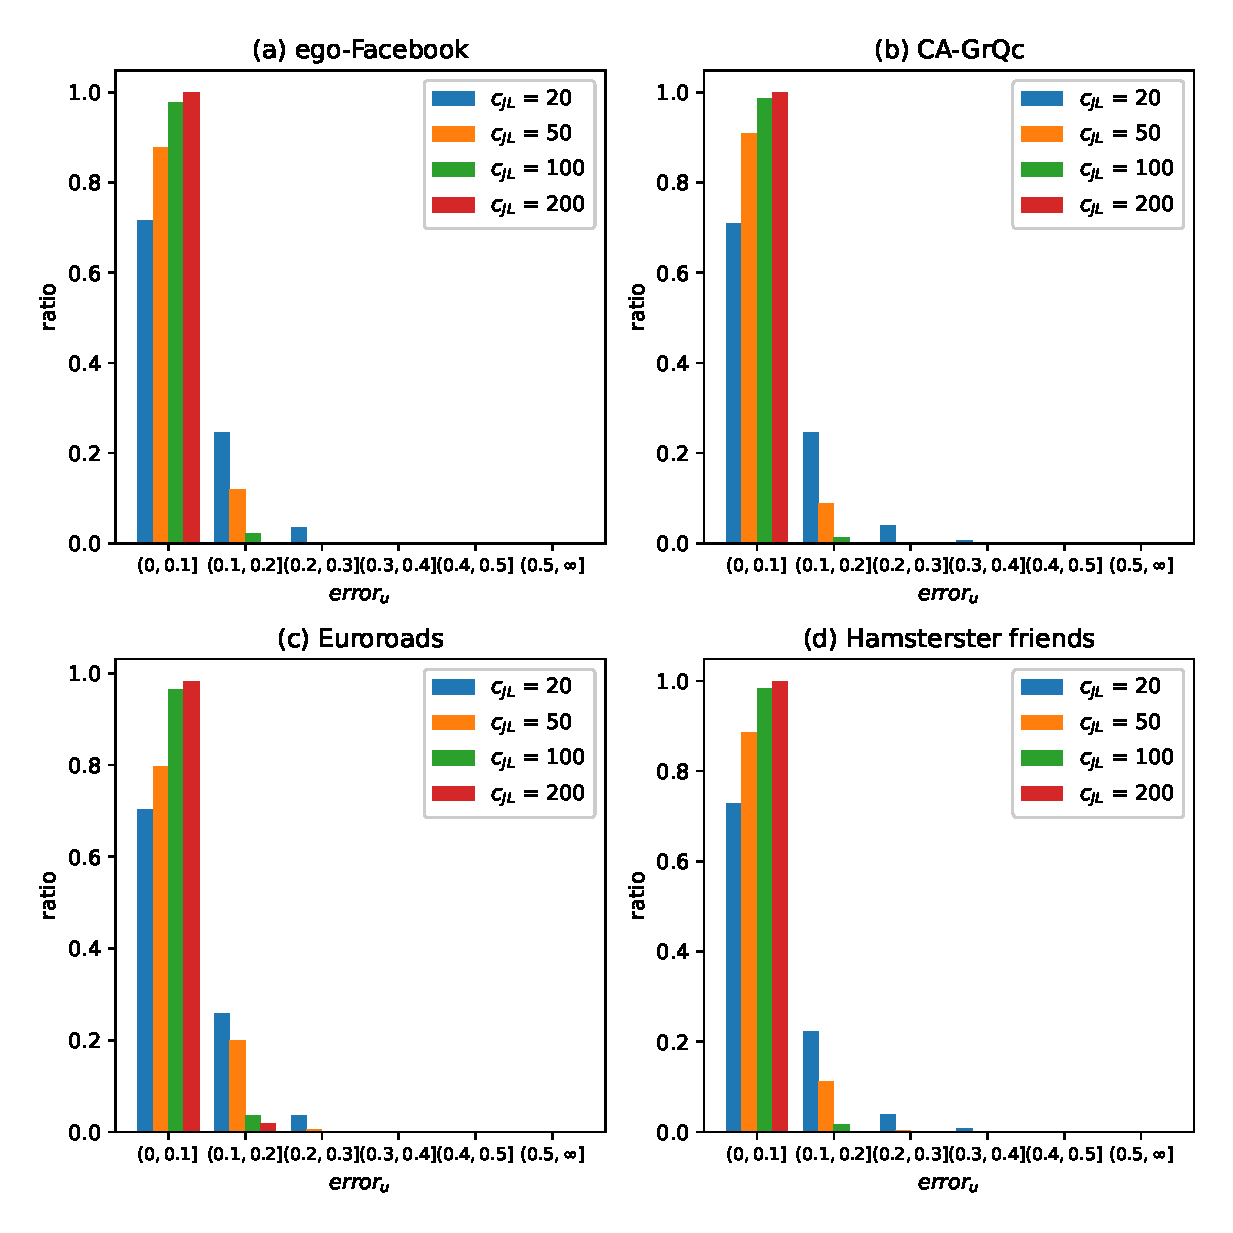
\includegraphics[width=0.475\textwidth]{margin_errors.eps}
    \caption{Relative error \(error_u\) distribution of algorithm \textsc{MarginEst} with different \(c_{JL}\) on four networks: ego-Facebook (a), CA-GrQc (b), Euroroads (c) and Hamsterster friends (d).\label{pic:margin-error}}
\end{figure}

\subsection{Performance of \textsc{Exact} and \textsc{Approx}}

Subsequently, we show the performance of proposed algorithms by comparing them with optimum solution and two other algorithms: \textsc{Top-SANC} and \textsc{Top-Degree} when solving MANC minimization problem.

We first compare the performance of \textsc{Exact} and \textsc{Approx} with optimum solution on four small networks.
For each network \(\gr=(V,E)\), we find the \(k\)-element set with minimum MANC value by enumerating all the \(k\)-element subsets of \(V\), then compare the minimum MANC value with solution given by \textsc{Exact} and \textsc{Approx}, whose results is shown in \figref{pic:compare-effect-optimum}.
\figref{pic:compare-effect-optimum} demonstrates that the solutions given by our greedy algorithms are almost the same with each other, both of them are also quite close to the optimum solution, which indicates that the approximation ratio of our proposed algorithms are far better than the theorecical guarantees.

\begin{figure}
    \centering
    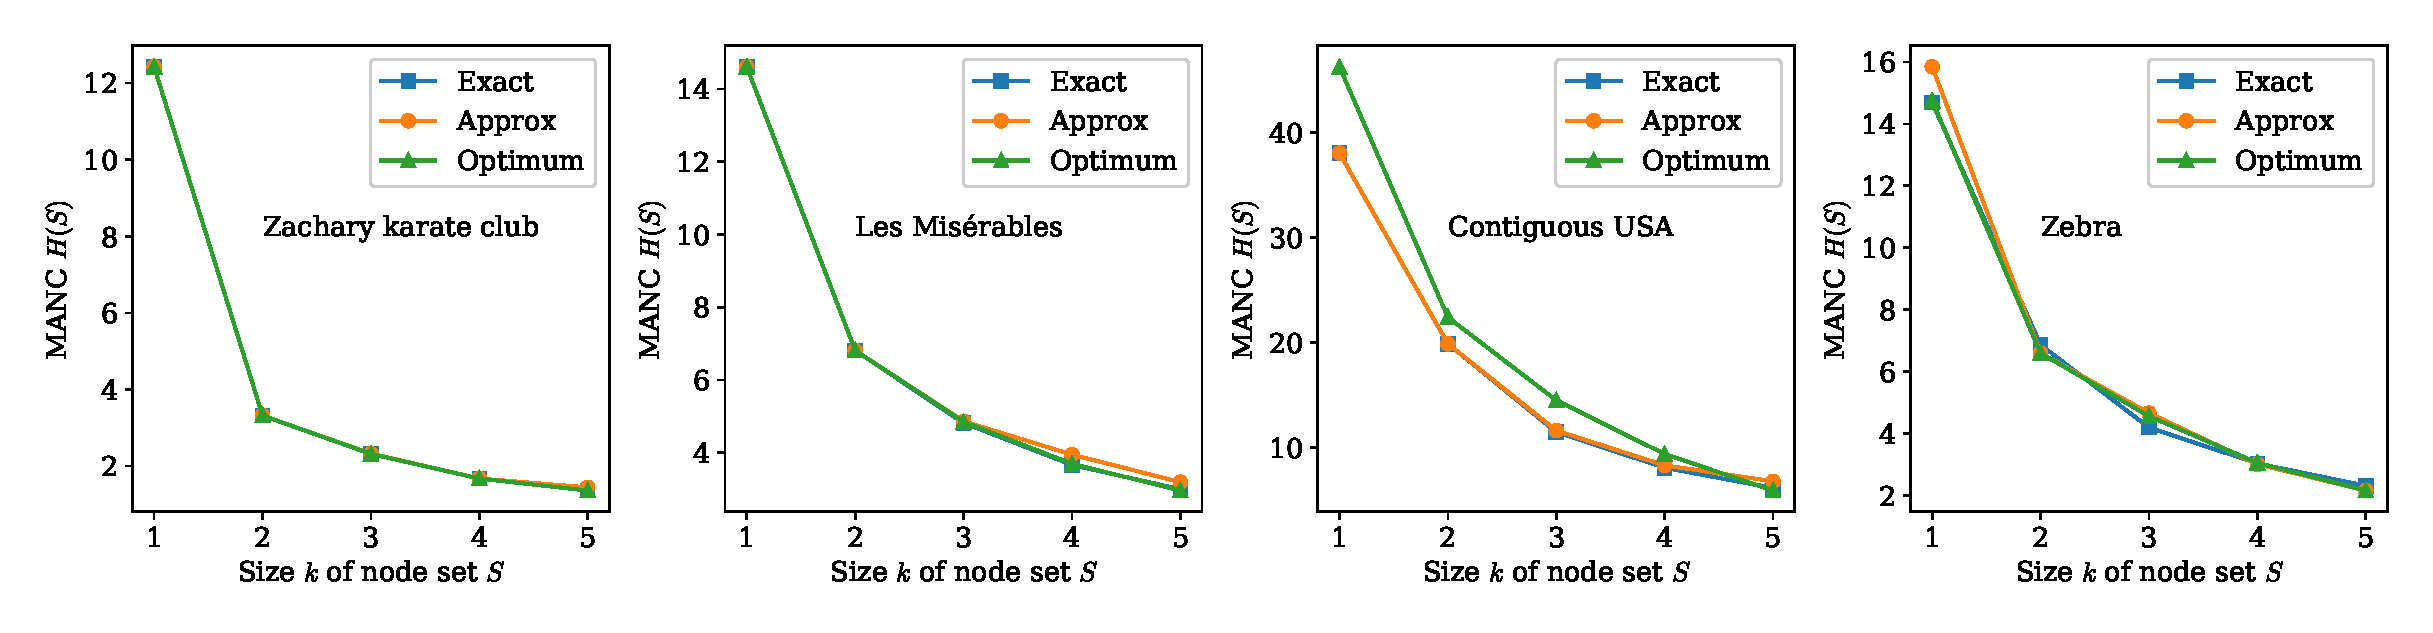
\includegraphics[width=0.475\textwidth]{compare_effects_optimum.eps}
    \caption{MANC \(M(S)\) of node set \(S\) computed by three different algorithms(\textsc{Exact},\textsc{Approx} and \textsc{Optimum}) on four networks: Zachary karate club (a), Les Misérables (b), Contiguous USA (c) and Zebra (d).\label{pic:compare-effect-optimum}}
\end{figure}

\textsc{Top-SANC} simply chooses \(k\) absorbing nodes with minimum SANC value which is defined in \secref{subsec:approx-margin-empty}, while \textsc{Top-Degree} chooses them with biggest degrees.
We run these four algorithms on four different real networks, the results is shown in \figref{pic:compare-effect}.
\figref{pic:compare-effect} demonstrates that both of our algorithms also get similar approximate solutions in larger networks, which outperform the solutions of other algorithms.

\begin{figure}
    \centering
    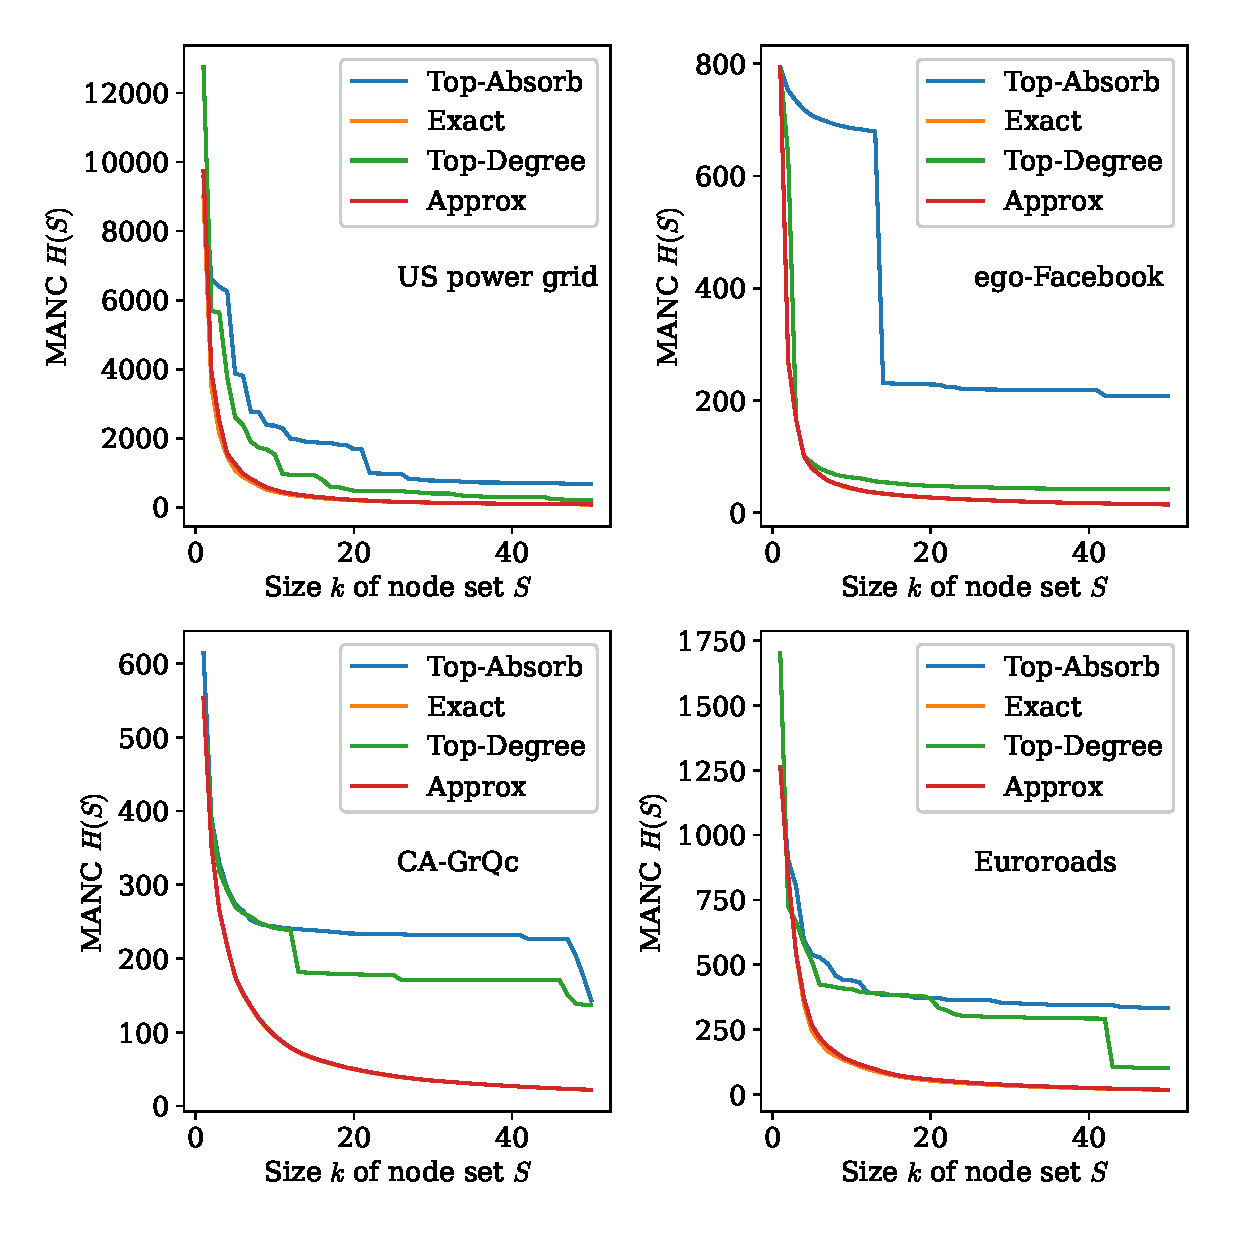
\includegraphics[width=0.475\textwidth]{compare_effects_exact.eps}
    \caption{MANC \(M(S)\) of node set \(S\) computed by four different algorithms(\textsc{Exact},\textsc{Approx},\textsc{Top-SANC} and \textsc{Top-Degree}) on four networks: US power grid (a), ego-Facebook (b), CA-GrQc (c) and Euroroads (d).\label{pic:compare-effect}}
\end{figure}

\subsection{Running time of \textsc{Exact} and \textsc{Approx}}

Finally, we prove that algorithm \textsc{Approx} is much more efficient than algorithm \textsc{Exact}, especially when applicated on large networks.
We test both algorithms on a larger set of real networks,.
For each network, we use \textsc{Exact} and \textsc{Approx} separately to solve MANC minimization problem, setting \(k=10\).
The running time of both algorithms is listed in \tabref{tab:running-time}.
From \tabref{tab:running-time}, we can observe that the running time of \textsc{Approx} is proportional to the number of edges in the network, thus leading to an increase in the speedup ratio of \textsc{Approx} compared to \textsc{Exact}as the network size grows.
In addition, \tabref{tab:running-time} indicates that \textsc{Approx} is still usable when dealing with networks with millions of nodes, while \textsc{Exact} fails because of its high time complexity.

\begin{table}
    \caption{The average running times and corresponding speedup ratio of \textsc{Exact} and \textsc{Approx} on a larger set of real networks.}
    \label{tab:running-time}
    \begin{tabular}{*4{c}}
        \toprule
        \multirow{2}*{Network} & \multicolumn{2}{c}{Time (seconds)} & \multirow{2}*{Speedup ratio}          \\
        \cmidrule(lr){2-3}     & \textsc{Exact}                     & \textsc{Approx}                       \\
        \midrule
        Euroroads              & 0.864                              & 0.509                        & 1.697  \\
        Hamsterster friends    & 2.679                              & 1.133                        & 2.365  \\
        ego-Facebook           & 39.499                             & 6.150                        & 6.423  \\
        CA-GrQc                & 42.611                             & 1.515                        & 28.126 \\
        US power grid          & 74.966                             & 1.530                        & 48.997 \\
        Reactome               & 139.377                            & 10.426                       & 13.368 \\
        CA-HepTh               & 392.903                            & 4.050                        & 97.013 \\
        Sister cities          & 667.902                            & 8.362                        & 79.873 \\
        CA-HepPh               & -                                  & 23.377                       & -      \\
        CAIDA                  & -                                  & 23.705                       & -      \\
        loc-Gowalla            & -                                  & 543.582                      & -      \\
        com-Amazon             & -                                  & 1643.860                     & -      \\
        Dogster friends        & -                                  & 3702.121                     & -      \\
        roadNet-PA             & -                                  & 8556.227                     & -      \\
        roadNet-CA             & -                                  & 17876.751                    & -      \\
        \bottomrule
    \end{tabular}
\end{table}

\section{Conclusions}

In this paper, we took the definition of hitting time of absorbing random walk as a basis, and extended it to the case to multiple nodes, i.e, Multiple Absorbing Node Centrality (MANC).
For a connected weighted undirected graph with \(n\) nodes and \(m\) edges, MANC \(M(S)\) of the node set \(S\) is defined as the weighted average of the hitting times of absorbing random walks from all nodes in the graph to \(S\).
Furthermore, we constructed the problem of finding the node set \(S^*\) with capacity \(k\) that minimizes \(M(S^*)\).
We proved that this problem is NP-hard, and the objective function is monotone and supermodular.
Due to these properties of MANC, we designed two approximate greedy algorithm, the former algorithm has a \(1-\frac1e\) approximate factor and \(O(kn^3)\) time complexity, while the latter algorithm obtains a \(1-\frac1e-\epsilon\) approximate factor and runs in time \(\tilde{O}(km)\).
Numerical experiments on real-world networks illustrate that both of the algorithms can provide solutions that are quite close to the optimal.
Specifically, numerical experiments on large networks incidate that the latter algorithm \textsc{Approx} is still well scalable while maintaining the approximation error and can be applicated in large networks with millions of nodes.

\bibliographystyle{ACM-Reference-Format}
\balance
\bibliography{main}

\end{document}